%!TEX root = ../Main.tex

% -----------------------------------------------------------------------------
\section{Results}
\label{s:Benchmarks}

We have implemented this system using Template Haskell for code generation in a library called @folderol@\footnote{\url{https://github.com/amosr/folderol}}.
To better compare against existing fusion systems, we have chosen to use the finite stream extension mentioned in~\S\ref{s:Finite} for our benchmarks.
We present three benchmarks: one array benchmark, and two file-based benchmarks.

\begin{figure}
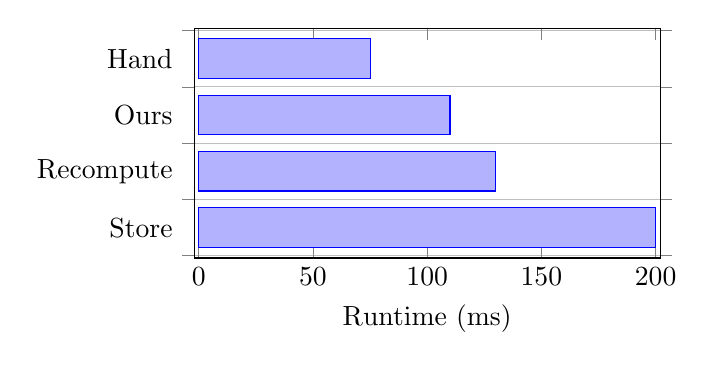
\begin{tikzpicture}
\begin{axis}[
  symbolic y coords={Store, Recompute, Ours, Hand, end},
	xlabel=Runtime (ms),
  xmin=0, xmax=200,
	enlargelimits=0.01,
	xbar interval=0.7,
  width=7.5cm, height=4.5cm,
	legend pos=north west,
]
\addplot coordinates {(200,Store) (130,Recompute) (110,Ours) (75,Hand) (0,end) };
\end{axis}
\end{tikzpicture}
\caption{Runtime for Quickhull; lower is faster.}
\label{fig:bench:quickhull}
\end{figure}

\subsection{Quickhull}
Quickhull is a divide-and-conquer spatial algorithm to find the smallest convex hull containing all points.
At its core is an operation called `filterMax', which takes a line and an array of points, and computes the maximum distance from the line, as well as all points that are above the line.
In our system this can be fused into a single loop, while shortcut-fusion systems do not support horizontal fusion.

We compare hand-fused against ours, as well as two @Data.Vector@ versions, which uses shortcut fusion.
The shortcut fusion system cannot fuse both operations into a single loop, and both operations require the distances between the line and each point.
This means a choice must be made: either compute the distances upfront and share them, or recompute the distances in each operation.
For our benchmarks we implemented both, and recomputing was significantly faster.
However, it is worth noting that we only benchmarked with two-dimensional points: at higher dimensions, the cost of recomputing distances may outweigh the cost of array allocation.

\autoref{fig:bench:quickhull} shows the runtimes for Quickhull over roughly 80MB of data, or five million points.
The hand-fused version is the fastest, while our version is slower, but still faster than the two vector versions.
The fact that our version is slower than the hand-fused version is surprising, as the generated GHC core is almost identical: the only difference is an extra continuation bound inside the loop, which acts as a sort of indirect jump in the recursive case.
It is possible that recent work on optimising continuations in GHC~\cite{downen2016sequent} will solve this.

\begin{figure}
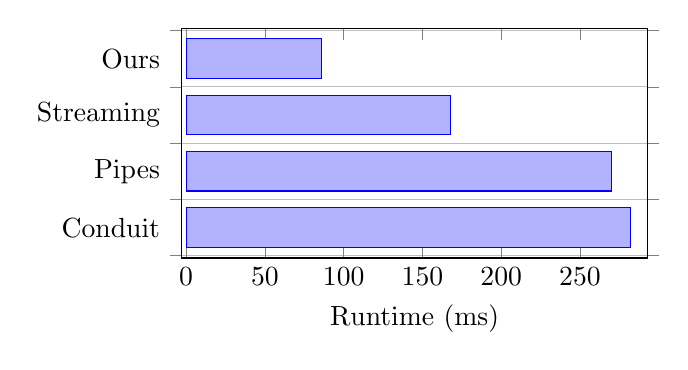
\begin{tikzpicture}
\begin{axis}[
  symbolic y coords={Conduit, Pipes, Streaming, Ours, end},
	xlabel=Runtime (ms),
  xmin=0, xmax=290,
	enlargelimits=0.01,
	xbar interval=0.7,
  width=7.5cm, height=4.5cm,
	legend pos=north west,
]
\addplot coordinates {(282,Conduit) (270,Pipes) (168,Streaming) (86,Ours) (0,end) };
\end{axis}
\end{tikzpicture}
\caption{Runtime for append2; lower is faster.}
\label{fig:bench:append}
\end{figure}

\subsection{Append files}
The first file-based benchmark consists of appending two files, while counting the number of lines.
We have benchmarked against three Haskell streaming libraries: Conduit, Pipes, and Streaming.
\autoref{fig:bench:append} shows the runtimes for appending 1.8MB of data.
The absolute performance here is poor because all are using line-buffered IO; in practice one would use chunked IO, but the overhead per chunk would remain.


\begin{figure}
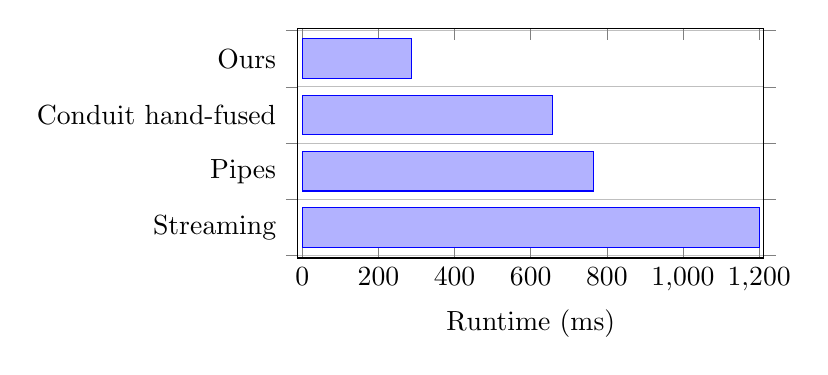
\begin{tikzpicture}
\begin{axis}[
  symbolic y coords={Streaming, Pipes, Conduit hand-fused, Ours, end},
	xlabel=Runtime (ms),
  xmin=0, xmax=1200,
	enlargelimits=0.01,
	xbar interval=0.7,
  width=7.5cm, height=4.5cm,
	legend pos=north west,
]
\addplot coordinates {(1200,Streaming) (764,Pipes) (658,Conduit hand-fused) (288,Ours) (0,end) };
\end{axis}
\end{tikzpicture}
\caption{Runtime for partition; lower is faster.}
\label{fig:bench:part}
\end{figure}

\subsection{Partition file}
The second file-based benchmark takes a single input file and partitions it into two files: one with even-length lines, and one with odd-length lines.
The number of lines in each output file is also counted.
The three streaming libraries are pull-based, and so do not support multiple outputs; the program must be written in a convoluted way or at least partially hand-fused.
Even with hand-fusion, the Pipes and Conduit programs are slower than ours, as well as losing any abstraction benefits from using a streaming library.
\autoref{fig:bench:part} shows the runtimes for partitioning a file into two.


